\chapter{Quantum Magnetism, Spinons and Kondo Physics}

Session 6 spent its whole runtime on magnets that break time-reversal symmetry: ferromagnets,
antiferromagnets, and, in its final stretch, the Holstein-Primakoff bosonization of these ordered
states into magnons, pushed all the way to a topological magnon band structure with its own
chiral edge modes. That session ended abruptly, right on ``topological magnons,'' with no closing
recap, but it did leave one loose thread along the way: a passing aside about Kitaev-type
interactions, flagged at the time as ``important for quantum spin liquids'' without being followed
up. This session is where that thread gets picked up properly, not as a resumed sentence but as
its own self-contained lecture, with its own welcome and its own roadmap: minimal models of
quantum magnetism, the excitations that quantum spin liquids (QSLs) support (spinons and gauge
excitations), and then Kondo systems and Kondo lattice models, where a completely different
physical setup turns out to be solvable with exactly the same trick. The thread that ties the
whole session together is the one that has been running under this entire course since session 1:
take a many-body Hamiltonian that mean-field theory cannot handle, find the right auxiliary-particle
reformulation, and mean-field \emph{that} instead.

We set $\hbar = 1$ throughout for the spin operators, matching the convention already implicit in
session 6.

\section{Two classes of magnet, and where each one lives}

Every magnetic material we could point to falls, in this lecture's language, into one of two
classes. \textbf{Classical magnets} break time-reversal symmetry: conventional ferromagnets,
antiferromagnets, spin spirals. From the electron's perspective these are describable by
mean-field theory, exactly as built in sessions 1 and 6, and this is where most magnetic materials
in nature actually sit: iron, copper oxide, or any material with a well-defined N\'eel temperature.

\textbf{Quantum magnets} are the opposite: they admit no mean-field description in terms of electrons at
all, and their ground states carry long-range entanglement. That entanglement is not a side detail,
it is what gives rise to excitations that have no counterpart in a symmetry-broken magnet. Two
quite different physical realizations of quantum magnetism are the subject of this session:

\begin{itemize}
\item \textbf{Quantum spin liquids (QSLs)}, the first class we build up in detail. The best-known candidate
  material is herbertsmithite, a compound whose magnetic ions sit on a kagome lattice of spin-$1/2$
  sites.
\item \textbf{Heavy-fermion Kondo insulators}, often rare-earth compounds, with samarium hexaboride
  (SmB$_6$) as the standard example. We build the theory for this class in the second half of the
  session.
\end{itemize}

\section{Two emergent excitations: magnons versus spinons}

Strong many-body interactions between electrons are what give magnetic materials their emergent,
collective excitations in the first place. In a symmetry-broken magnet, that collective excitation
is the \textbf{magnon}: spin $1$, no charge, because the strong electronic repulsion freezes the charge
degree of freedom completely and only spin is left to fluctuate. In a quantum magnet, the
excitation is qualitatively different: the \textbf{spinon}, spin $1/2$, also no charge. It is useful to
picture a spinon as literally the spin half of an electron. Push that picture one step further and
you get the standard fractionalization language for a QSL: the electron splits into a \textbf{chargon},
carrying the charge, and a \textbf{spinon}, carrying the spin.

There is a simple pictorial argument for why the two excitations differ by exactly a factor of two
in spin. Take a ferromagnet: the ground state is all spins up, $|{\uparrow\uparrow\uparrow\cdots}\rangle$.
Flip one spin to build an excited state, and the difference in total spin between ground and
excited state is $\Delta S = 1$: a (local) magnon. Now take a quantum spin liquid: the ground state
is a collection of singlets everywhere, no single spin pointing anywhere in particular. Build an
excited state by leaving one spin unpaired instead of pairing it into a singlet, and the difference
in total spin is $\Delta S = 1/2$: pictorially, a spinon. This picture is deliberately oversimplified
(spinons are genuinely more subtle than ``an unpaired spin''), but it is exactly the right starting
intuition for why symmetry-broken magnets and quantum spin liquids host fundamentally different
excitations. Figure~\ref{fig:s08:magnonspinon} puts the two counting arguments side by side.

% Session 8 -- magnon versus spinon: the Delta S = 1 versus Delta S = 1/2 counting.
% Placement: sec. "Two emergent excitations: magnons versus spinons", right after the
% "simple pictorial argument" paragraph.
%
% NOTE (physics): a chain of an even number of sites cannot host a single unpaired
% spin, so the excited singlet background is drawn with the honest *two* unpaired
% sites. The point of the figure survives unchanged and gets sharper: each unpaired
% spin separately carries S=1/2, which is exactly why the elementary excitation is
% half a magnon rather than a whole one.
\begin{aqmfigure}{fig:s08:magnonspinon}{Why the two kinds of magnet host excitations differing by
exactly a factor of two in spin. (a) In a symmetry-broken magnet every site carries a definite spin
(arrows). Flipping one costs $\Delta S=1$: that excitation is the magnon of session 6. (The single flipped
spin drawn here is only the $\Delta S$ bookkeeping; the actual magnon is the delocalized precession
of figure~\ref{fig:s06:magnon}, not one overturned site.) (b) In a
quantum magnet no site carries a definite spin at all; the sites are paired into singlets (8.3)
(capsules), so $\langle\mathbf S_i\rangle=0$ everywhere and $S_\text{tot}=0$. Breaking one pair
leaves \emph{unpaired} sites (open circles), and each one separately carries $S=1/2$: a spinon,
half a magnon. Spinons are therefore always created in pairs, and whether the pair stays bound or
comes apart is the whole content of figure~\ref{fig:s08:vbsrvb}.}

\begin{tikzpicture}[x=1cm, y=1cm]

\tikzset{
  sup/.pic={\draw[aqm, -{Stealth[length=3.8pt,width=3.2pt]}] (0,-0.21) -- (0,0.21);},
  sdn/.pic={\draw[aqm, -{Stealth[length=3.8pt,width=3.2pt]}] (0,0.21) -- (0,-0.21);},
  chainline/.style={aqm, draw=aqmmuted, line width=\aqmthinwidth},
  capsule/.style={aqm, draw=aqmaccent, fill=aqmfill, rounded corners=0.19cm},
  dot/.style={aqmsite, minimum size=4.6pt},
  dotopen/.style={aqmsite, fill=white, draw=aqmbroken, minimum size=6.5pt,
                  line width=\aqmlinewidth}
}

\def\dx{0.62}
\def\xa{-0.42}   % right edge of the left label column
\def\xr{5.05}    % left edge of the right annotation column

% ======================= (a) symmetry-broken magnet =========================
\node[aqmpanel, anchor=west] at (\xa-2.55,0.98) {(a) symmetry-broken magnet};

% --- ground state -----------------------------------------------------------
\draw[chainline] (-0.12,0) -- (7*\dx+0.12,0);
\foreach \n in {0,...,7} {
  \node[dot] at (\n*\dx,0) {};
  \pic at (\n*\dx,0.36) {sup};
}
\node[aqmlabsmall, anchor=east, text=aqmmuted] at (\xa,0.18) {ground state};
\node[aqmlabsmall, anchor=west] at (\xr,0.18)
  {$S_\text{tot}^z=N/2$, \; $\langle S_i^z\rangle=\tfrac12$ on every site};

% --- one flipped spin -------------------------------------------------------
\draw[chainline] (-0.12,-1.10) -- (7*\dx+0.12,-1.10);
\foreach \n in {0,...,7} { \node[dot] at (\n*\dx,-1.10) {}; }
\foreach \n in {0,1,2,4,5,6,7} { \pic at (\n*\dx,-0.74) {sup}; }
\draw[aqm, draw=aqmbroken, line width=\aqmthinwidth, dash pattern=on 1.8pt off 1.6pt,
      rounded corners=2pt, fill=white]
  (3*\dx-0.17,-0.99) rectangle (3*\dx+0.17,-0.49);
\pic[draw=aqmbroken] at (3*\dx,-0.74) {sdn};
\node[aqmlabsmall, anchor=east, text=aqmmuted] at (\xa,-0.92) {flip one spin};
\node[aqmlabsmall, anchor=west, align=left] at (\xr,-0.92)
  {$\Delta S = 1$: \textbf{magnon} \; \textcolor{aqmmuted}{(spin $1$, no charge)}};

% ======================= (b) quantum magnet =================================
\node[aqmpanel, anchor=west] at (\xa-2.55,-2.05) {(b) quantum magnet};

% --- singlet-covered ground state -------------------------------------------
\foreach \n in {0,2,4,6} {
  \draw[capsule] (\n*\dx-0.19,-2.94) rectangle (\n*\dx+\dx+0.19,-2.56);
}
\foreach \n in {0,...,7} { \node[dot] at (\n*\dx,-2.75) {}; }
\node[aqmlabsmall, anchor=east, text=aqmmuted, align=right] at (\xa,-2.75)
  {ground state:\\[-1pt]every site paired};
\node[aqmlabsmall, anchor=west, align=left] at (\xr,-2.75)
  {$S_\text{tot}=0$, \; $\langle \mathbf S_i\rangle=\mathbf 0$ on every site};

% --- one pair broken --------------------------------------------------------
\foreach \n in {0,3,6} {
  \draw[capsule] (\n*\dx-0.19,-4.09) rectangle (\n*\dx+\dx+0.19,-3.71);
}
\foreach \n in {0,1,3,4,6,7} { \node[dot] at (\n*\dx,-3.90) {}; }
\foreach \n in {2,5} { \node[dotopen] at (\n*\dx,-3.90) {}; }
\node[aqmlabsmall, anchor=north, text=aqmbroken] at (2*\dx,-4.06) {$S=\tfrac12$};
\node[aqmlabsmall, anchor=north, text=aqmbroken] at (5*\dx,-4.06) {$S=\tfrac12$};
\node[aqmlabsmall, anchor=east, text=aqmmuted, align=right] at (\xa,-3.90)
  {break one pair};
\node[aqmlabsmall, anchor=west, align=left] at (\xr,-3.90)
  {$\Delta S = \tfrac12$ each: \textbf{spinon} \; \textcolor{aqmmuted}{(spin $\tfrac12$, no charge)}};

% --- legend for the capsule --------------------------------------------------
\node[aqmlabsmall, anchor=north west, text=aqmmuted] at (\xa-2.55,-4.55)
  {capsule $=$ singlet $\tfrac{1}{\sqrt2}\big(|{\uparrow\downarrow}\rangle-|{\downarrow\uparrow}\rangle\big)$
   of (8.3); \; open circle $=$ unpaired site};

\end{tikzpicture}

\end{aqmfigure}


\section{Two minimal dimers: classical order parameter versus quantum singlet}

The cleanest way into quantum magnetism is to look first at the smallest possible magnet, two
spins, and compare two different Hamiltonians on it.

The first is the \textbf{Ising dimer},

\begin{equation}
\mathcal H_\text{Ising} = S_0^z S_1^z,
\end{equation}

coupling only the $z$-components of two spin-$1/2$'s. This Hamiltonian has two degenerate ground
states, related by time reversal:

\begin{equation*}
|GS_1\rangle = |{\uparrow\downarrow}\rangle, \qquad |GS_2\rangle = |{\downarrow\uparrow}\rangle.
\end{equation*}

Both are eigenstates with the same energy, but each one \emph{individually} breaks time-reversal
symmetry (time reversal flips every spin, so it swaps $|GS_1\rangle$ and $|GS_2\rangle$ into one
another); only the two-state degenerate pair together respects it. A macroscopic, symmetry-broken
antiferromagnet, of exactly the kind built in session 6, is just an infinite-site version of this
same story, and the same argument runs equally well for ferromagnets and spin spirals.

Now replace the Ising coupling by the full, rotationally symmetric \textbf{quantum Heisenberg dimer},

\begin{equation}
\mathcal H_\text{Heis} = \mathbf S_0 \cdot \mathbf S_1.
\end{equation}

This is what a half-filled, strongly-interacting Hubbard model reduces to in the large-$U$ limit
(session 1's derivation). Solving it with $\mathbf S_0, \mathbf S_1$ as genuine spin-$1/2$
operators, two spin-$1/2$'s combine into a singlet ($S=0$) and a triplet ($S=1$), with
$\mathbf S_0\cdot\mathbf S_1 = -3/4$ on the singlet and $+1/4$ on the triplet, so the unique ground
state is the \textbf{singlet},

\begin{equation}
|GS\rangle = \frac{1}{\sqrt2}\Big(|{\uparrow\downarrow}\rangle -
|{\downarrow\uparrow}\rangle\Big), \qquad \langle \mathbf S_i \rangle = 0.
\end{equation}

This ground state is qualitatively different from the Ising case in three ways that matter for
everything that follows: it is \emph{uniquely} the ground state, with no degeneracy to spontaneously
choose between; it is \emph{time-reversal symmetric}, since its net magnetization vanishes on the nose
and time reversal maps $|GS\rangle$ to itself; and it is \emph{maximally entangled} (the two terms in
(8.3) carry equal weight, the largest entanglement two qubits can hold). Can we have a macroscopic
version of this same ground state? That question is exactly where quantum spin liquids come from.

\section{Frustration: the route to a quantum spin liquid}

Before building a macroscopic version of (8.3), we need to know when a Heisenberg model's ground
state actually stays time-reversal symmetric like this, rather than spontaneously ordering the way
session 1 and session 6's magnets did. The rule of thumb is \textbf{frustration}. The paradigm case is a
triangular plaquette with antiferromagnetic coupling on all three bonds: any two spins can point
oppositely, but the third bond is then forced to sit between two spins that are already
antiparallel to each other, and no single spin configuration satisfies all three bonds at once.
Geometric frustration of this kind produces many classically degenerate ground states (same energy,
different spin configurations), and once quantum fluctuations are switched on, they mix these
degenerate configurations into a single quantum superposition that, generically, does not break
time-reversal symmetry.

This is why the \textbf{triangular} and \textbf{kagome} lattices, both built entirely out of triangles, are
the standard hunting ground for quantum spin liquid physics: an antiferromagnetic Heisenberg model
on either lattice is, in the right coupling regime, a genuine candidate for a QSL ground state. And
this is precisely why herbertsmithite, a kagome-lattice compound of spin-$1/2$ sites, keeps coming
up as the best-known real material candidate. Figure~\ref{fig:s08:frustration} collects the geometry
behind the whole argument: an unfrustrated plaquette, a frustrated triangle with its degenerate
configurations, and the kagome lattice built entirely out of them.

% Session 8 -- geometric frustration: the degenerate Ising triangle and the kagome lattice.
% Placement: sec. "Frustration: the route to a quantum spin liquid", after the
% triangular-plaquette paragraph.
% Rendered by figures/blender/s08f02_frustration.py, labels in figures/overlays/s08f02_frustration.tex.
\begin{aqmfigure}{fig:s08:frustration}{Frustration, with the spins drawn as Ising (collinear)
variables, which is how the argument in the text is written. If the spins can rotate freely, the
triangle goes instead into the $120^\circ$ noncollinear state of figure~\ref{fig:s06:frustration},
and the degeneracy that we discuss here is the Ising one. The plaquette without frustration and the
single frustrated triangle are panels (a) and (b) of figure~\ref{fig:s06:frustration}. On a
bipartite plaquette every antiferromagnetic bond can be satisfied at the same time, and the ground
state is the N\'eel state, with two configurations related by a global flip, each of which breaks
time-reversal symmetry. On a triangle this is not possible, since once two spins are antiparallel
the third bond cannot be satisfied for both directions of the last spin. (a) The frustrated bond, in
red, can be on any of the three edges, so the classical ground state is degenerate and not unique.
Quantum fluctuations mix the degenerate configurations into one superposition with $\langle\mathbf
S_i\rangle=\mathbf 0$, which does \emph{not} break time-reversal symmetry. (b) The kagome lattice of
herbertsmithite is built only from corner-sharing triangles, so all of them are frustrated at the
same time, here with one frustrated bond on every triangle, and the classical degeneracy becomes
macroscopic. This is why triangular and kagome lattices are the standard place to look for quantum
spin liquids.}
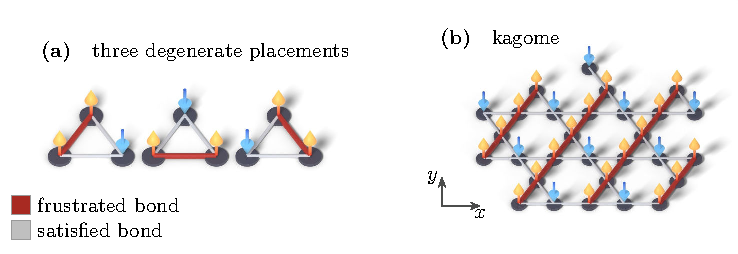
\includegraphics{figures/pdf/s08f02_frustration.pdf}
\end{aqmfigure}


\section{A first stop short of a spin liquid: the dimerized Heisenberg model}

Before tackling a genuinely frustrated Hamiltonian, it is worth building the simplest possible
\emph{macroscopic} quantum magnet and checking explicitly that its ground state does what (8.3) promised.
Take a \textbf{fully dimerized Heisenberg model}: perfectly decoupled dimers, arranged in a chain or on
a two-dimensional lattice,

\begin{equation}
H = \sum_n J\, \mathbf S_{2n}\cdot \mathbf S_{2n+1}, \qquad J>0.
\end{equation}

Because every dimer is completely decoupled from its neighbors, the many-body ground state can be
written down exactly, as a simple product of singlets over the dimer pairs,

\begin{equation}
|\Psi\rangle \sim \bigotimes_n \Big(|{\uparrow_{2n}\downarrow_{2n+1}}\rangle -
|{\downarrow_{2n}\uparrow_{2n+1}}\rangle\Big), \qquad \langle \mathbf S_i\rangle = 0 \text{ on every
site}.
\end{equation}

This is, in one sense, a trivial Hamiltonian, effectively a collection of independent
zero-dimensional problems. But it already establishes something important: a macroscopic Heisenberg
Hamiltonian genuinely \emph{can} have a ground state that does not break time-reversal symmetry, exactly
generalizing the two-site singlet (8.3) to an extensive system. Turning on small couplings between
the dimers deforms this state smoothly without breaking time-reversal symmetry either.

There is, however, a crucial distinction to draw here, because this state is \emph{not yet} a quantum
spin liquid. Its fundamental excitations are still spin-$1$ excitations: break one singlet into its
triplet partner, and you get a \textbf{triplon}, a local singlet-to-triplet transition, structurally the
same object as a magnon in everything but name. A state built this way, out of a fixed, static
pattern of singlets, is called a \textbf{valence bond solid (VBS)}. Getting to a genuine quantum spin
liquid, with spin-$1/2$ excitations rather than spin-$1$ triplons, requires going a step further
than a static dimer covering: it requires the singlets themselves to fluctuate and resonate across
the whole lattice, which is exactly the frustrated case we return to next.
Figure~\ref{fig:s08:vbsrvb} draws that contrast explicitly.

\section{The QSL ground state: the resonating valence bond wavefunction}

For a genuinely frustrated Heisenberg Hamiltonian $\mathcal H = \sum_{ij} J_{ij}\, \mathbf
S_i\cdot\mathbf S_j$, the expected ground state is no longer a single, fixed dimer covering like
(8.5). Instead it is a \textbf{linear combination of singlets over every possible pairing of sites}, each
pairing carrying its own amplitude, a genuinely complicated many-body wavefunction. One could try to
attack this directly (write it as a tensor network, as session 7 does for the general strongly
correlated case), but there is a more physically transparent route: a variational ansatz built on an
analogy to superconductivity.

The idea is that singlets in a QSL ``feel'' a lot like Cooper pairs in an s-wave superconductor: both
are pairwise singlet correlations. A BCS-type wavefunction is easy to write at the mean-field level
in the right basis (Nambu space, exactly as in session 5), so we start from a BCS-paired state built
out of the same auxiliary fermions $f_{i\sigma}$ that we will justify properly in Section 8.8,

\begin{equation}
|\Psi_\text{BCS}\rangle = \prod_{\mathbf k}\Big(u_{\mathbf k} + v_{\mathbf k}\,
f^\dagger_{\mathbf k\uparrow} f^\dagger_{-\mathbf k\downarrow}\Big)|0\rangle,
\end{equation}

with $u_{\mathbf k}, v_{\mathbf k}$ variational parameters exactly as in session 5's BCS state. Left
on its own, (8.6) is a superposition of states with every possible fermion occupation per site
(empty, singly, doubly occupied), which is not a physical spin state at all: a QSL enforces strong
local interactions, so single occupation per site is required, with no charge fluctuations allowed
between sites. We enforce this by applying a \textbf{Gutzwiller projector} onto the singly-occupied
subspace,

\begin{equation}
|\Psi_\text{RVB}\rangle = P_G\,|\Psi_\text{BCS}\rangle, \qquad P_G = \prod_i n_i(2-n_i), \qquad
n_i = \sum_\sigma f^\dagger_{i\sigma}f_{i\sigma},
\end{equation}

which evaluates to $1$ on states with exactly one fermion per site and to $0$ otherwise. What
survives is a genuine many-body spin wavefunction: a superposition over ways of pairing up sites
into singlets, in the spirit of the single-dimer singlet (8.3), now spread across an entire
frustrated lattice. This construction is named exactly for what it describes: the \textbf{resonating
valence bond (RVB)} variational wavefunction, and it turns out to be a genuinely good description
of quantum spin liquid physics. Figure~\ref{fig:s08:vbsrvb} shows what separates this resonating
state, and the excitations it supports, from the frozen dimer covering of Section 8.5.

% Session 8 -- valence bond solid versus resonating valence bond: a fixed dimer covering
% Placement: end of sec. "The QSL ground state: the resonating valence bond wavefunction",
% referenced from the dimerized-Heisenberg section as well.
% Rendered by figures/blender/s08f03_vbs_rvb.py, labels in figures/overlays/s08f03_vbs_rvb.tex.
\begin{aqmfigure}{fig:s08:vbsrvb}{The difference between a valence bond solid and a quantum spin
liquid is not whether the ground state is built from singlets, since both are, but whether the
singlet pattern is frozen. (a1) The fully dimerized model (8.4) has one fixed covering, (8.5). (a2)
When we separate the two unpaired spins of figure~\ref{fig:s08:magnonspinon}b, every strong bond
between them loses its singlet, drawn in red, so the energy cost grows with the separation. The pair
is confined, and only the bound object propagates, which is the spin-$1$ triplon. (b1) The RVB state
(8.7) is a superposition over \emph{all} pairings, near and far, drawn as coverings stacked on top
of each other. (b2) Now the background pairs again behind the excitations with no cost, the
confining string does not form, and the two halves separate as independent spin-$1/2$ spinons.
Frustration is the reason why the superposition in (b1), and not a single covering, is the ground
state.}
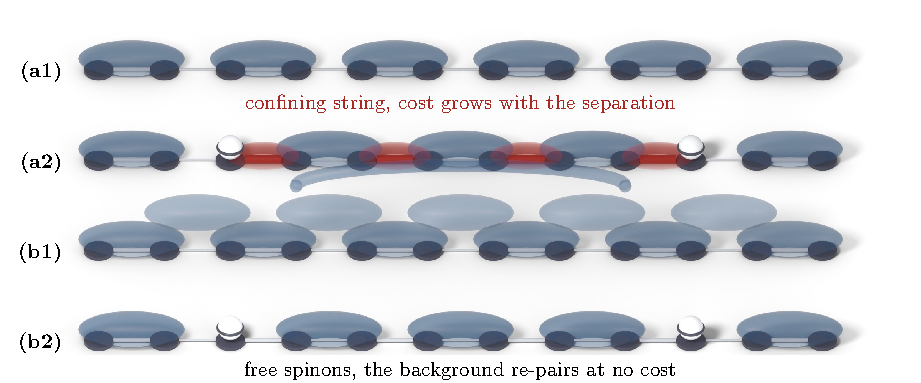
\includegraphics{figures/pdf/s08f03_vbs_rvb.pdf}
\end{aqmfigure}


\section{Why the magnon (Holstein-Primakoff) approach fails for QSL excitations}

Writing down the exact QSL ground state is hard, so the natural next move, exactly as in session 6,
is to ask about excitations \emph{on top of} the ground state rather than the ground state itself. Our
only tool for that so far is the \textbf{Holstein-Primakoff transformation}, which represents

\begin{equation}
S_i^z = S - a_i^\dagger a_i, \qquad S_i^+ \approx \sqrt{2S}\,a_i, \qquad S_i^- \approx
\sqrt{2S}\,a_i^\dagger,
\end{equation}

linearized under the assumption that the bosonic magnon population is small,
$\langle a_i^\dagger a_i\rangle \ll S$: an excellent approximation near a fully (or nearly)
polarized magnet, exactly the regime session 6 used it in.

A QSL sits in the opposite limit. Its defining property, $\langle \mathbf S_i\rangle = 0$ on every
site, forces, through (8.8),

\begin{equation}
\langle a_i^\dagger a_i \rangle = S,
\end{equation}

precisely the regime where the small-boson-density condition behind the linearized
Holstein-Primakoff mapping fails outright. There is no ordered reference state for a QSL to be
``close to'' and expand around, so the whole magnon machinery that worked for session 6's ordered
magnets simply is not the right tool here. We need a genuinely different approximation for the
excitations of a quantum spin liquid.

\begin{notebookbox}{\texttt{session8.ipynb}, ``Magnetization of a large Heisenberg model'' (Core)}
Diagonalize a moderately large quantum Heisenberg chain and confirm numerically that the local
magnetization stays zero on every site, even in the presence of a small external field, as long as
that field is weaker than the finite-size gap to the neighboring total-spin sector: the numerical
face of the defining property behind (8.4) and (8.9).
\end{notebookbox}

\section{The parton construction: Abrikosov fermions and the single-occupancy constraint}

The construction that makes QSL excitations tractable represents each spin not as a bosonic
fluctuation around an ordered reference state, but as an auxiliary \textbf{fermion} field $f_{i\sigma}$
($\sigma=\uparrow,\downarrow$) living at every site: a particle carrying spin $1/2$ but no electric
charge, exactly the spinon of Section 8.2, now written down formally. These are called
\textbf{Abrikosov fermions}, and the operator identity that defines the parton transformation is

\begin{equation}
\mathbf S_i = \frac12 \sum_{\alpha\beta} f_{i\alpha}^\dagger\, \boldsymbol\sigma_{\alpha\beta}\,
f_{i\beta},
\end{equation}

with $\boldsymbol\sigma$ the vector of Pauli matrices. One can check directly, from the fermionic
anticommutation relations, that (8.10) reproduces the correct $SU(2)$ spin algebra
$[S_i^a,S_i^b] = i\varepsilon^{abc}S_i^c$ on the full four-state Fock space of
$f_{i\uparrow},f_{i\downarrow}$ (empty, singly occupied up, singly occupied down, doubly occupied),
with no extra input needed. The catch is that this transformation \emph{artificially enlarges} the local
Hilbert space: a physical spin-$1/2$ has only two states, while $f_{i\uparrow},f_{i\downarrow}$
give four. We remove the two unphysical extra states (empty and doubly occupied, both of which
(8.10) sends to $\mathbf S_i=0$ anyway) by imposing, by hand, the \textbf{single-occupancy constraint}

\begin{equation}
\sum_\sigma f_{i\sigma}^\dagger f_{i\sigma} = 1 \qquad \text{at every site } i.
\end{equation}

This is exactly the fermionic analogue of the Gutzwiller projection (8.7) applied earlier to the
many-body wavefunction: projecting the many-body state onto the singly-occupied subspace and
constraining the fermion filling to one per site are the same statement, seen from the wavefunction
side versus the operator side. Figure~\ref{fig:s08:parton}a shows exactly which two states the
constraint has to throw away, and why they were never spin states to begin with.

With (8.11) enforced, (8.10) is an \emph{exact} rewriting of a spin-$1/2$ operator in fermionic language,
and we can substitute it directly into the Heisenberg Hamiltonian $\mathcal H=\sum_{\langle
ij\rangle}J_{ij}\,\mathbf S_i\cdot\mathbf S_j$. Using the Pauli-matrix Fierz identity
$\sum_a \sigma^a_{\alpha\beta}\sigma^a_{\gamma\delta} = 2\delta_{\alpha\delta}\delta_{\beta\gamma} -
\delta_{\alpha\beta}\delta_{\gamma\delta}$ and the constraint (8.11) on both sites gives the clean
identity

\begin{equation}
\mathbf S_i \cdot \mathbf S_j = \frac14 - \frac12\, \chi_{ij}^\dagger \chi_{ij}, \qquad \chi_{ij}
\equiv \sum_\sigma f_{i\sigma}^\dagger f_{j\sigma},
\end{equation}

with $\chi_{ij}$ the spinon ``bond'' (hopping) operator between sites $i$ and $j$. Substituting (8.12)
turns the original, bilinear-in-spin Heisenberg Hamiltonian into a Hamiltonian that is \emph{quartic} in
the auxiliary fermions,

\begin{equation}
\mathcal H = \sum_{\langle ij\rangle} J_{ij}\left(\frac14 - \frac12\,\chi_{ij}^\dagger\chi_{ij}\right)
= \text{const} - \frac12\sum_{\langle ij\rangle} J_{ij}\, \chi_{ij}^\dagger \chi_{ij}.
\end{equation}

This is exactly the same kind of difficulty session 1 and session 6 faced with the electronic
Hubbard interaction: a quartic term with no direct diagonalization. We treat it the same way, by
\textbf{mean-field decoupling},

\begin{equation}
\chi_{ij}^\dagger\chi_{ij} \;\approx\; \langle\chi_{ij}^\dagger\rangle\,\chi_{ij} +
\chi_{ij}^\dagger\,\langle\chi_{ij}\rangle - |\langle\chi_{ij}\rangle|^2.
\end{equation}

\section{The mean-field spinon Hamiltonian and its dispersion classes}

Absorbing the couplings and expectation value of (8.14) into a single mean-field parameter
$\chi_{ij}$ per bond, and enforcing the constraint (8.11) on average with a Lagrange multiplier if
needed, the mean-field decoupling of Section 8.8 collapses the original spin problem into a genuine,
diagonalizable tight-binding-like Hamiltonian for the auxiliary fermions,

\begin{equation}
\mathcal H_\text{MF} = \sum_{ij,s} \chi_{ij}\, f^\dagger_{i,s} f_{j,s}.
\end{equation}

It is worth pausing on what makes this mean-field step different from every other mean-field
decoupling in this course so far: it does not need to break time-reversal symmetry. Choosing the
same $\chi_{ij}$ for spin up and spin down keeps $\langle \mathbf S_i\rangle = 0$ exactly, so the
resulting ground state is time-reversal symmetric by construction, just as (8.4) and (8.9) require.
Equation (8.15) is nothing but a tight-binding model for the auxiliary fermions, with hoppings
$\chi_{ij}$ fixed self-consistently by the lattice geometry and the exchange couplings $J_{ij}$. Its
excitations are the \textbf{spinons}: emergent, spin-$1/2$, charge-neutral fermionic quasiparticles,
produced by exactly the same ``quartic interaction, mean-field decouple, diagonalize a bilinear
Hamiltonian'' recipe used for electrons throughout this course, just transplanted into the spin
sector. Figure~\ref{fig:s08:parton}b is the resulting picture: spinons hopping on the lattice with
amplitude $\chi_{ij}$, at half filling because of (8.11).

% Session 8 -- the parton construction: an enlarged local Hilbert space, cut back down
% Placement: sec. "The parton construction", after the single-occupancy constraint (8.11).
% Rendered by figures/blender/s08f04_parton.py, labels in figures/overlays/s08f04_parton.tex.
\begin{aqmfigure}{fig:s08:parton}{What the Abrikosov-fermion rewriting (8.10) costs, and what it
gives us. (a) The four fermionic states of a site. The two singly-occupied states give the physical
spin-$1/2$ doublet exactly. The empty and doubly-occupied states, drawn as ghosts with a cross, are
extra unphysical states, which (8.10) maps to $\mathbf S_i=\mathbf 0$ and which the constraint
(8.11) removes by hand, and this constraint is the operator version of the Gutzwiller projector
(8.7). (b) What remains after the mean-field decoupling (8.14), which is an ordinary tight-binding
problem (8.15) for fermions with spin-$1/2$ and no charge, which hop with the self-consistent bond
amplitude $\chi_{ij}$, drawn as the thickness of the bond, here with two values for illustration.
Since there is one fermion per site, the resulting spinon model must be studied at half filling.
Taking the same $\chi_{ij}$ for both spin species keeps $\langle\mathbf S_i\rangle=\mathbf 0$, so
this mean field, unlike the magnetic mean fields of sessions 1 and 6, does not break time-reversal
symmetry.}
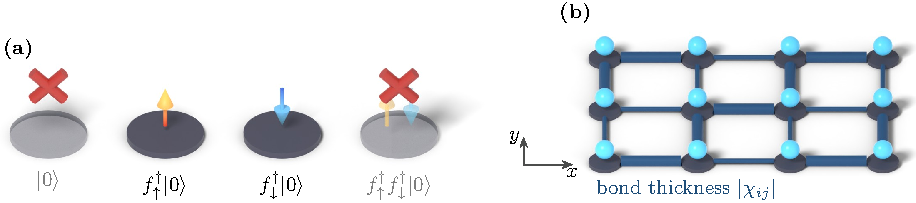
\includegraphics{figures/pdf/s08f04_parton.pdf}
\end{aqmfigure}


Diagonalizing (8.15) on a given lattice produces a genuine spinon band structure, and depending on
the resulting mean-field parameters, three qualitatively different outcomes are possible:

\begin{itemize}
\item \textbf{Gapless spinons}, with excitations arbitrarily close to zero energy.
\item \textbf{Gapped spinons}, with a finite energy cost to create a spinon.
\item \textbf{Dirac spinons}, with a linear energy-momentum relation at isolated points in the Brillouin
  zone.
\end{itemize}

\begin{notebookbox}{\texttt{session8.ipynb}, ``Spinon Fermi surface in gapless quantum spin liquids'' (Core)}
Build the spinon tight-binding Hamiltonian (8.15) on the triangular lattice and watch its Fermi
surface evolve as the ratio of hopping amplitudes $t_2/t_1$ changes. The quiz asks you to redo it
on the square and kagome lattices, and to justify why the effective spinon model must sit at half
filling: that is exactly the single-occupancy constraint (8.11) at the mean-field level.
\end{notebookbox}

\section{Emergent gauge symmetry and vison excitations}

There is one more essential piece to the QSL story, and it is a direct consequence of the fact that
we introduced fermions to represent a spin. Consider a local, site-dependent phase rotation of the
auxiliary fermions,

\begin{equation}
f_{i\sigma} \;\to\; e^{i\theta_i}\, f_{i\sigma}, \qquad f^\dagger_{i\sigma} \to e^{-i\theta_i}
f^\dagger_{i\sigma}.
\end{equation}

Both the physical spin operator (8.10) and the single-occupancy constraint (8.11) are completely
unaffected by (8.16): the phase $e^{i\theta_i}$ cancels between $f^\dagger_{i\alpha}$ and
$f_{i\beta}$ in every term, so the Hamiltonian and the physical spin operators are exactly invariant.
But the mean-field bond variable $\chi_{ij}$ is \emph{not}: it picks up a relative phase,
$\chi_{ij} \to e^{i(\theta_i - \theta_j)}\chi_{ij}$. This is precisely the structure of a lattice
gauge theory: $\chi_{ij}$ behaves like a link variable, and (8.16) is a local (``gauge'')
transformation under which the physical spin theory is invariant while the mean-field saddle point
of Section 8.9 is not. Any two choices of $\chi_{ij}$ related by (8.16) describe exactly the same
physical quantum spin liquid; the mean-field decoupling only ever fixes a gauge-equivalence class,
not a unique set of hoppings. This redundancy is the origin of an \textbf{emergent gauge theory} for
quantum spin liquids.

Once this gauge structure is recognized, $\chi_{ij}$ becomes a genuinely dynamical field on the
lattice links, capable of carrying its own topological defects, in direct analogy to how the
superconducting order parameter's gauge degree of freedom can host vortices. Write the mean-field
Hamiltonian as $\mathcal H = \sum_{ij,s}|\chi_{ij}|e^{i\theta_{ij}}f^\dagger_{i,s}f_{j,s}$, and
define the flux around a plaquette as the product of phases picked up going around its boundary,
$\Phi = \prod e^{i\theta_{ij}}$. A concrete example: on a square lattice, imagine hoppings around
every elementary loop pick up phase $\Phi=+1$ (a ground state), except one loop, which picks up
$\Phi=-1$. That single flipped plaquette is an excited state, a topological defect in the emergent
gauge field, called a \textbf{vison}: the gauge sector's own excitation, generally coupled to the matter
sector's spinon excitations built in Section 8.9. A quantum spin liquid, in this language, is
characterized not just by its spinon dispersion but by an emergent gauge theory and the vison
excitations that theory supports, a genuinely new organizing principle with no counterpart anywhere
in the symmetry-broken magnets of session 6. There is no notebook exercise built around this
construction; it stands as a purely conceptual, formal piece of the QSL picture.
Figure~\ref{fig:s08:gauge} draws both halves of it: why the flux, and not the link variable, is the
physical quantity, and what a single flipped flux looks like on the lattice.

% Session 8 -- the emergent gauge structure: link phases are gauge-dependent, plaquette
% Placement: sec. "Emergent gauge symmetry and vison excitations", after the square-lattice
% example.
% Rendered by figures/blender/s08f05_gauge_vison.py, labels in figures/overlays/s08f05_gauge_vison.tex.
\begin{aqmfigure}{fig:s08:gauge}{The emergent gauge theory of the parton construction, and its
excitation, seen from above. (a) The mean-field bond variable is defined on the links,
$\chi_{ij}=|\chi_{ij}|e^{i\theta_{ij}}$, drawn as a dial at the phase $\theta_{ij}$, and the local
phase rotation (8.16) on one site shifts every link phase by $\theta_i-\theta_j$, which changes the
two red needles. When we go once around a plaquette, each site phase appears twice with opposite
signs, so the flux $\Phi=\prod e^{i\theta_{ij}}$ does not change. The link variables are pure gauge,
and the flux is physical. This is the reason why two mean-field solutions related by (8.16) describe
the same spin liquid. (b) As a result, the flux is what labels the state. With $\Phi=+1$ on every
plaquette as the ground state, flipping a single plaquette to $\Phi=-1$ costs energy, and no gauge
transformation can remove it. This localized defect of the gauge field is a \textbf{vison}. Which
links have the minus sign is a gauge choice, here a string from the edge, and it can be moved
freely, while the shaded plaquette cannot be moved.}
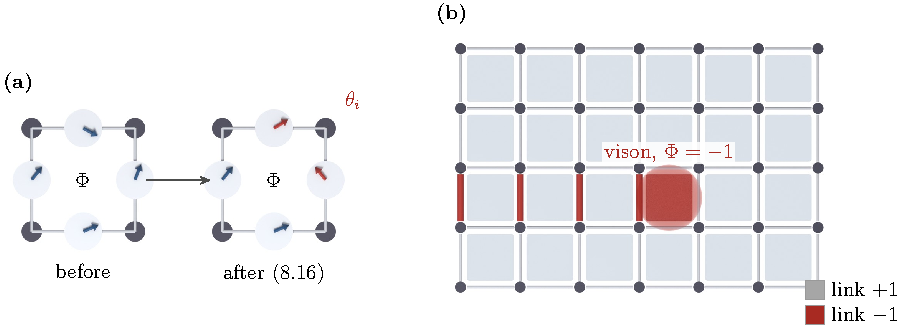
\includegraphics{figures/pdf/s08f05_gauge_vison.pdf}
\end{aqmfigure}


\section{From a single Kondo impurity to the Kondo lattice}

Having built the machinery for quantum spin liquids, the lecture turns to a second, physically quite
different setting that turns out to be solvable with exactly the same trick: the \textbf{Kondo lattice
model}, which arises whenever a metal and a correlated, local-moment system coexist.

Start with the simplest possible case: a single spin-$1/2$ magnetic impurity sitting inside a
non-interacting two-dimensional electron gas. The total Hamiltonian is a free, dispersive kinetic
term for the conduction electrons, plus a Heisenberg-like coupling between the impurity spin and the
local conduction-electron spin density at the impurity site,

\begin{equation}
H = -t\sum_{\langle ij\rangle,\sigma}\Big(c^\dagger_{i\sigma}c_{j\sigma} + \text{h.c.}\Big) +
H_K, \qquad H_K = \sum_{\alpha\beta}\Big(c^\dagger_{0\beta}\,\boldsymbol\sigma_{\beta\alpha}\,
c_{0\alpha}\Big)\cdot \mathbf S,
\end{equation}

the \textbf{Kondo coupling} $H_K$. Solving this exactly is a genuinely hard many-body problem, but the
physical picture of its ground state is simple to state even without the full solution: the impurity
spin forms a singlet, structurally the same object as (8.3), with some effective conduction electron
in its vicinity,

\begin{equation*}
|GS\rangle \sim \frac{1}{\sqrt2}\Big(|{\Uparrow\downarrow}\rangle -
|{\Downarrow\uparrow}\rangle\Big),
\end{equation*}

while the rest of the electron gas behaves as an effectively non-interacting Fermi sea. This turns
out to be a genuinely good approximation to the many-body ground state, and the resulting state has
total spin zero and does not break time-reversal symmetry: despite hosting a real local moment,
this is already, in the sense of Section 8.4, a quantum magnet.

Now generalize to a whole \textbf{lattice} of magnetic impurities, one per site, each coupled to the same
conduction-electron bath,

\begin{equation}
H = -t\sum_{\langle ij\rangle,\sigma}\Big(c^\dagger_{i\sigma}c_{j\sigma} + \text{h.c.}\Big) +
J\sum_{j,\alpha\beta}\Big(c^\dagger_{j\beta}\,\boldsymbol\sigma_{\beta\alpha}\,c_{j\alpha}\Big)\cdot
\mathbf S_j.
\end{equation}

Every impurity again wants to form a singlet with a nearby conduction electron, but with many
impurities competing for the same electron sea, the screening electrons end up shared, fractionally,
between different impurities' singlets. The result is a state of massive, lattice-wide entanglement
between all the magnetic sites and the electron gas, while the total spin remains exactly zero.

\begin{notebookbox}{\texttt{session8.ipynb}, ``Magnetization of a large Heisenberg model with a magnetic impurity'' (Challenge) and ``Magnetization of a dimerized Heisenberg model with a magnetic impurity'' (Challenge)}
These exercises show, numerically and in real space, how a single magnetic impurity's local field
decays with distance into an otherwise gapless or dimerized quantum magnet: the gapless chain shows
algebraic, staggered decay, tracing the correlation profile of a critical spin liquid; the
dimerized (valence-bond-solid) chain of Section 8.5 instead shows exponential decay over a finite
correlation length, because its ground state is gapped. This is the same screening-cloud physics
behind (8.17), viewed from the real-space, single-chain side rather than the itinerant-electron
side.
\end{notebookbox}

\section{Solving the Kondo lattice: the same parton trick, now with a hybridization}

The lecture makes the parallel to Section 8.8 explicit: this problem is solved the same way we
solved the QSL. Replace every impurity spin by an Abrikosov fermion, $\mathbf S_j = \tfrac12
f_{j\alpha}^\dagger \boldsymbol\sigma_{\alpha\beta} f_{j\beta}$, subject to the same single-occupancy
constraint (8.11), written here in the equivalent traceless form

\begin{equation}
S_{\alpha\beta}(j) = f^\dagger_{j\alpha}f_{j\beta} - \frac{n_f(j)}{N}\delta_{\alpha\beta}.
\end{equation}

Substituting into (8.18) turns the Kondo coupling into a genuine quartic interaction, now coupling
the auxiliary $f$ fermions not to another site's $f$ fermion (as in (8.13)) but to the \emph{real}
conduction electrons $c_{j\sigma}$ at the same site,

\begin{equation}
H \sim \sum_{\mathbf k\alpha} \varepsilon_{\mathbf k}\, c^\dagger_{\mathbf k\alpha}c_{\mathbf
k\alpha} \;-\; J\sum_{j,\alpha\beta}\Big(c^\dagger_{j\beta}f_{j\beta}\Big)\Big(f^\dagger_{j\alpha}
c_{j\alpha}\Big).
\end{equation}

Exactly as in (8.14), we mean-field decouple this quartic term, taking the expectation value
$\langle c^\dagger_j f_j\rangle$, and Fourier transform to momentum space. This produces a genuinely
bilinear Hamiltonian mixing real electrons and auxiliary fermions,

\begin{equation}
H \sim \sum_{\mathbf k\alpha} \varepsilon_{\mathbf k}\, c^\dagger_{\mathbf k\alpha} c_{\mathbf
k\alpha} \;-\; \gamma_K \sum_{\mathbf k,\alpha\beta} f^\dagger_{\mathbf k\alpha}c_{\mathbf k\alpha} +
\text{h.c.},
\end{equation}

with $\varepsilon_{\mathbf k}$ the \textbf{conduction band dispersion} and $\gamma_K$ the \textbf{Kondo
hybridization}, the single self-consistently determined mean-field parameter carrying all of the
information about the strength of the original Kondo coupling $J$.

\section{Electronic structure of the Kondo lattice: the Kondo insulator}

Equation (8.21) is, per spin, an ordinary two-band Bloch Hamiltonian in the basis $(c_{\mathbf
k\alpha}, f_{\mathbf k\alpha})$. When $\gamma_K = 0$, there is no mixing at all: the spectrum is
simply the ordinary, dispersive conduction band $\varepsilon_{\mathbf k}$, together with a
perfectly \textbf{flat}, zero-energy band of $f$-fermion levels (flat because these auxiliary fermions
carry no hopping of their own once the Kondo coupling is switched off). Switching the Kondo coupling
back on makes $\gamma_K$ finite, and the flat and dispersive bands undergo an \textbf{anti-crossing}:
wherever the flat spinon band would have crossed the conduction band, a \textbf{gap} opens instead, and
the bigger the Kondo coupling, the bigger this gap becomes. This is confirmed directly by comparing
the spectra at increasing $J_K$: at $J_K=0$ the bands simply cross; already by $J_K=0.25$ a visible
gap has opened at the crossing; by $J_K=0.5$ the gap is substantially larger.
Figure~\ref{fig:s08:kondobands} shows the two ends of that comparison, and where the Fermi level
sits in each.

% Session 8 -- the Kondo lattice band structure: a flat f level anti-crossing a conduction
% Placement: sec. "Electronic structure of the Kondo lattice: the Kondo insulator", after
% the anti-crossing paragraph.
% Rendered by figures/blender/s08f06_kondo_bands.py, labels in figures/overlays/s08f06_kondo_bands.tex.
\begin{aqmfigure}{fig:s08:kondobands}{Why a lattice of local moments is an insulator, drawn from
(8.21) per spin in one dimension. (a) With the Kondo coupling switched off, (8.21) is a dispersive
conduction band $\varepsilon_{\mathbf k}$ together with a completely flat band of $f$ levels, the
red line. This band is flat because the auxiliary fermions have no hopping of their own, and the two
bands cross at the Fermi level, which gives a metal. (b) A finite hybridization $\gamma_K$ removes
the crossing. The bands repel each other, the states close to the crossing become mixtures of
conduction electron and local moment, and a gap opens exactly where the crossing was. With one $f$
fermion per site from the constraint (8.11) and a half-filled conduction band, the lower hybridized
band is exactly full. So the Fermi level is inside the gap, and the metal has become a \textbf{Kondo
insulator}. The gap grows with $\gamma_K$, and so with the Kondo coupling $J_K$, and the nearly flat
band edges that remain are the reason why the remaining quasiparticles are heavy.}
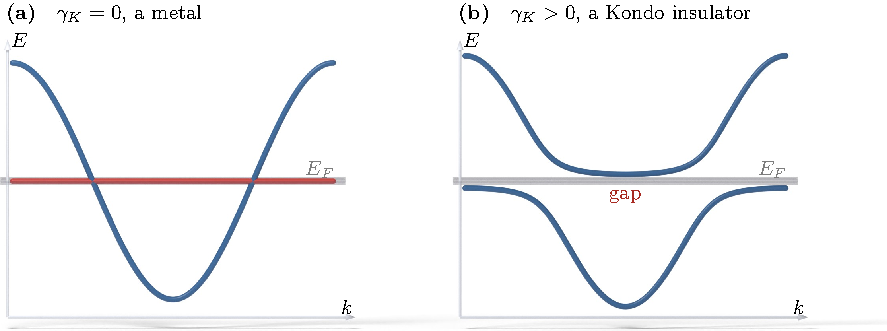
\includegraphics{figures/pdf/s08f06_kondo_bands.pdf}
\end{aqmfigure}


Physically, the ground state of this hybridized system is, by construction, non-magnetic:
total spin zero, time-reversal symmetric, exactly as it was for the single impurity (8.17) and for
the quantum spin liquid of Section 8.9. The consequence for the electronic structure, though, is
new: a lattice of Kondo impurities converts what would otherwise be an ordinary metal into an
\textbf{insulator}, because every electron sitting at the Fermi surface ends up forming a bound state
with a magnetic impurity. This is the \textbf{Kondo insulator}, also called a heavy-fermion insulator,
and SmB$_6$, introduced already in Section 8.1, is the standard real-material example.

It is worth noting the resemblance to a rather different construction from session 5: superconductors
also open a gap in their quasiparticle spectrum through hybridization, there between electrons and
holes rather than between electrons and auxiliary fermions. The two settings are physically very
different, but the \emph{mechanism} by which the single-particle spectrum develops a gap is closely
analogous, and so is the way the effect turns on: the temperature scale at which the Kondo-insulator
gap becomes visible depends on the Kondo coupling in a strongly non-linear way, the same qualitative
non-linear dependence familiar from the superconducting gap's dependence on the pairing interaction.

\begin{notebookbox}{\texttt{session8.ipynb}, ``Quantum magnetism in the Kondo lattice'' (Core) and ``Spinon dispersion in the Kondo lattice'' (Challenge)}
The first exercise builds (8.21) directly on a van der Waals-type lattice: identify the flat
(Kondo-site) band, the anti-crossing with the conduction band, and check what happens to the gap as
you move the chemical potential. The second adds a direct exchange coupling between the Kondo
sites themselves, giving the otherwise-flat spinon band its own dispersion, the lattice version of
the Doniach picture: the Kondo coupling $J_K$ favors a local screened singlet while the direct
exchange $J$ favors magnetic correlations between the local moments, and their competition controls
which regime, screened or magnetic, is stable.
\end{notebookbox}

\section{Closing summary}

The lecture's own closing recap, reconstructed here with the equations it was pointing back to:

\begin{itemize}
\item Magnetism, in every form met across sessions 1, 6 and today, arises from strong repulsive
  interactions between electrons.
\item Frustrated magnetic models (triangular and kagome lattices, Section 8.4) can display \textbf{quantum
  spin liquid} behavior: a ground state with zero local spin expectation value on every site (8.4),
  maximally entangled, generalizing the Heisenberg dimer singlet (8.3) through the valence-bond-solid
  state (8.5) to a genuinely resonating, frustrated ground state (8.6)-(8.7); conventional mean-field
  theory cannot capture it by construction.
\item Because a QSL's zero magnetization is the opposite regime from the one Holstein-Primakoff needs
  (8.9), its fundamental excitations are not magnons but \textbf{spinons}, with $S=1/2$: emergent,
  charge-neutral fermions obtained from the Abrikosov/parton construction, (8.10)-(8.15), the
  electron mean-field recipe of sessions 1 and 6 transplanted into the spin sector. Spinon bands can
  be gapless, gapped, or Dirac-like (Section 8.9).
\item The parton construction carries an emergent gauge redundancy (8.16): the mean-field bond variable
  is a link field whose topological defects are gauge excitations called \textbf{visons}, generally
  coupled to the spinons (Section 8.10).
\item Quantum entanglement mixing spin and fermion degrees of freedom also arises in \textbf{Kondo systems}:
  the same parton trick, applied to a lattice of local moments embedded in a metal, (8.17)-(8.21),
  turns the Kondo exchange coupling into a mean-field \textbf{hybridization} $\gamma_K$ that gaps the
  conduction band at the anti-crossing and converts a metal into a \textbf{Kondo insulator}
  (heavy-fermion insulator), with the gap growing monotonically with the Kondo coupling strength
  (Section 8.13).
\end{itemize}

Session 9 picks this construction straight back up: the Abrikosov-fermion/spinon machinery built
here gets reused directly, now applied to a single magnetic impurity sitting inside an otherwise
ordinary metal, with an explicit callback to a Friedel-oscillation result derived earlier in that
same session.
